\subsection{Irrational Guards Are Sometimes Needed \cite{abrahamsen2021art}}
This paper \cite{abrahamsen2021art} studies the placement of the guards in the context of The Art Gallery Problem \cite{o1987art}. Namely, it focusses on and confirms that there are polygons with integer coordinates that require guards placed at points with irrational coordinates. Generalising, this paper shows that $\forall n \in \mathbb N$, there is a family of simple monotone polygons that can either be guarded by $3n$ guards with irrational coordinates, or $4n$ guards with rational coordinates. The result is also extended to a rectilinear polygon that can be guarded by 9 guards with irrational coordinates, or 10 guards with rational coordinates. The family of simple monotone polygons that can be guarded by $3n$ guards with irrational coordinates, as well as the rectilinear polygon that can be guarded by 9 guards with irrational coordinates are also discussed.


At the time of writing the paper, there was no combinatorial algorithm for finding an optimal solution for The Art Gallery Problem \cite{o1987art}, nor for its decidability version on whether a set $S$ of given size $k$ exists. As such, it is not known whether the problem is in NP.

First, we will address the question regarding whether polygons given by integer coordinates require guard positions with irrational coordinates in any optimal solution by introducing a crafted monotone polygon $\mathcal P$. A polygon is monotone if there exists a line $l$ such that every line orthogonal to $l$ intersects it at most twice. $\mathcal P$ is depicted in Figure \ref{fig:p} and is constructed using a rectangle, six triangular pockets (in green), three rectangular pockets (in blue) and four quadrilaterial pockets (in red) are added. The intuition behind the polygon will be explained in the upcoming subsections. The figure is accredited to \cite{1057165}.

\begin{figure}[h!]
    \centering
    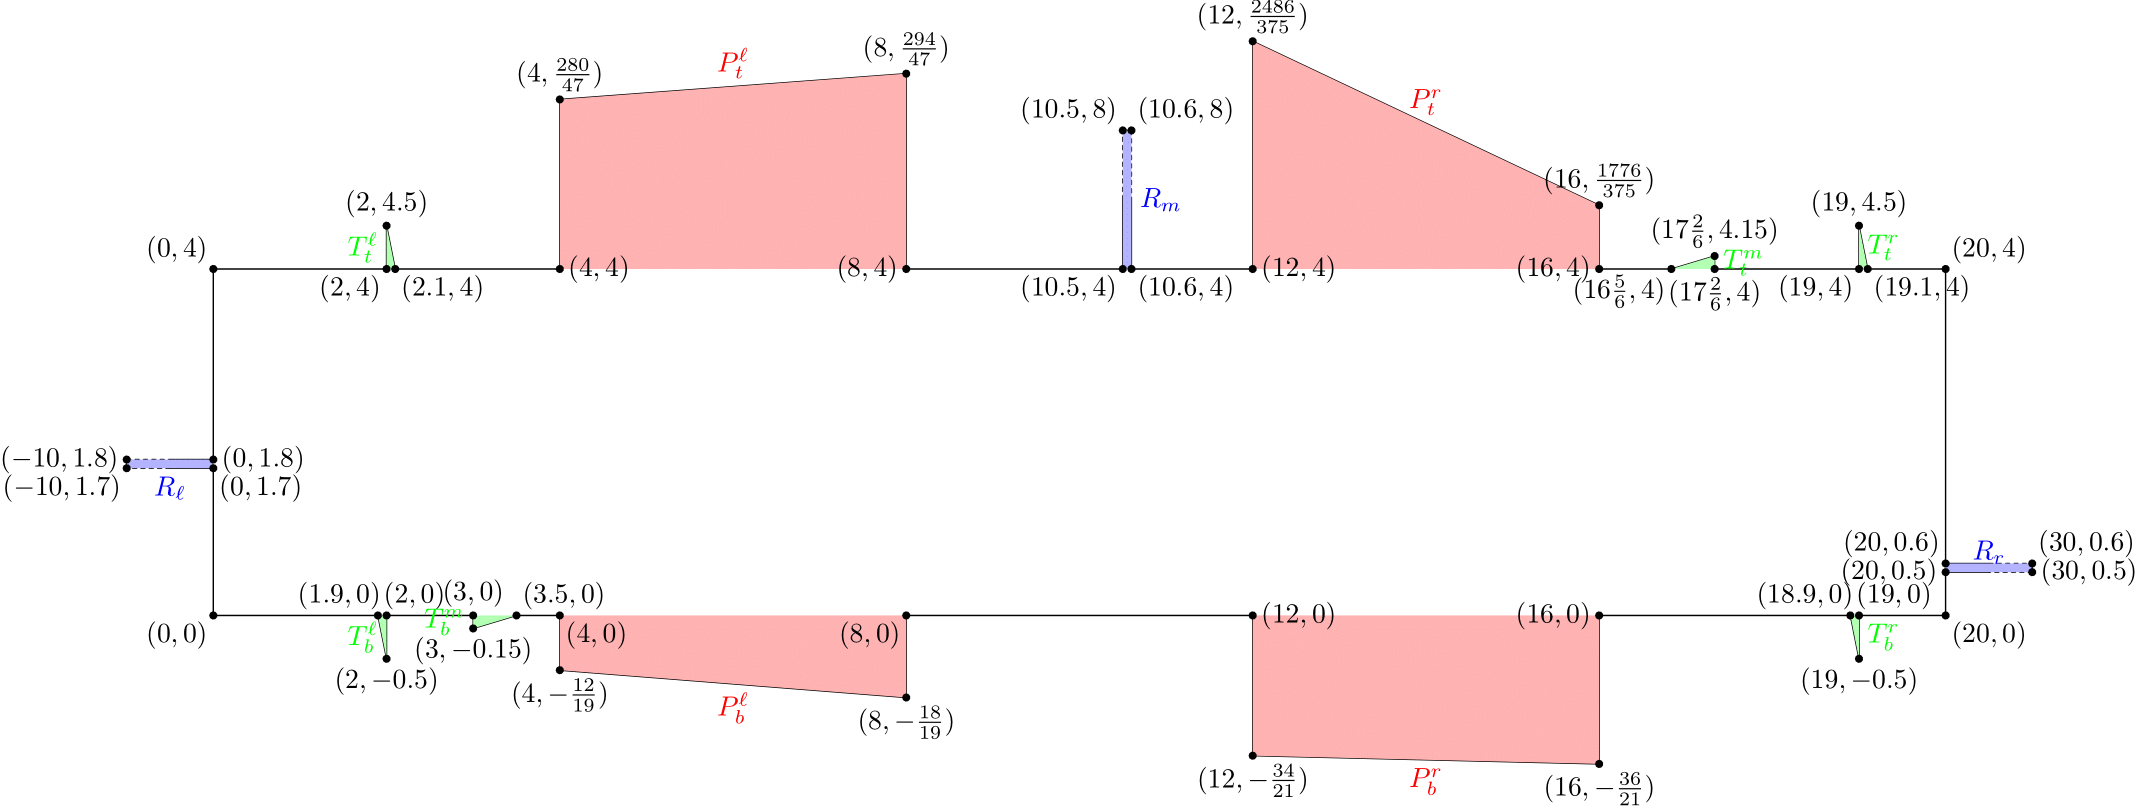
\includegraphics[width=\textwidth]{fig-12-1.png}
    \caption{Polygon $\mathcal P$}
    \label{fig:p}
\end{figure}

\subsubsection{Intuition for Triangular Pockets}
The six triangular pockets are created in order to force a guard on a line segment. As such, they are grouped into three pairs: top pockets are paired with bottom pockets corresponding to their position in $\mathcal P$. A depiction of this positioning can be found in Figure \ref{fig:tb} (b). For every pair (leftmost, middle, rightmost) of triangular pockets, there is a corresponding line $l_\ell, l_m, l_r$, respectively, that joins the peaks of each triangular pocket in a pair. A guard can see both the peaks $t, b$ of the pockets only if it is placed on the line segment $\overline{tb}$ (Figure \ref{fig:tb} (a)). Hence, one guard is needed per pair, resulting in 3 guards in total.

\begin{figure}[h!]
    \centering
    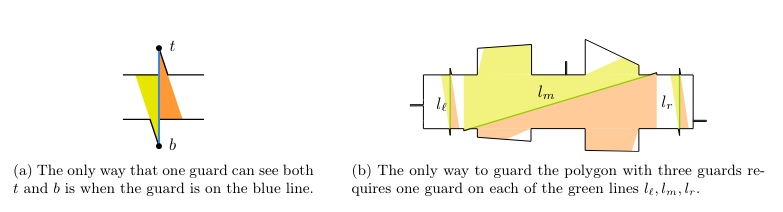
\includegraphics[width=\textwidth]{Screenshot from 2022-02-02 09-57-44.png}
    \caption{Forcing Guards to Lie on Specific Line Segments.}
    \label{fig:tb}
\end{figure}

\subsubsection{Intuition for Quadrilaterial Pockets}
The four quadrilateral pockets are created in order to force a guard in a region bounded by a curve. Figure \ref{fig:quadrilateral_pockets} depicts the visualisation for this case. Considering the fixed position of a guard $g_m$ either on the left or on the right of the curve $c_\ell$, there exists a position of guard $g_\ell$ on $l_\ell$ such that edge $e_t^\ell$ and line $p_b^{\ell}g_m$ are seen by $g_\ell$. Then, only if $g_m$ is on the left or on $c_\ell$ can it see the remaining parts of the pockets that are not seen by $g_\ell$ (edge $e_b^{\ell}$, line $p_t^{\ell}g_{\ell}$). Analogously, in order for the right side of $\mathcal P$ and the right pair of quadrilateral pockets to be seen by both guards $g_m$ and $g_r$, $g_m$ has to be on the curve $c_r$ or on its right. Since $g_m$ has to also satisfy its position on $c_\ell$, its only feasible position is as the intersection point between $c_\ell$ and $c_r$. 

\begin{figure}[h!]
    \centering
    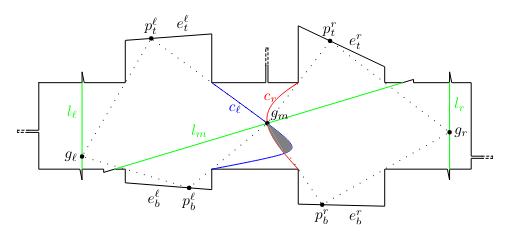
\includegraphics[width=0.7\textwidth]{Screenshot from 2022-01-21 12-02-44.png}
    \caption{Restricting a Guard to a Region Bounded by a Curve}
    \label{fig:quadrilateral_pockets}
\end{figure}

\subsubsection{Intuition for Rectangular Pockets}
The three rectangular pockets are created in order to force a guard to a single irrational point. Further building onto the previously discussed instance from Figure \ref{fig:quadrilateral_pockets}, the three rectangular pockets on the laterals and top of $\mathcal P$ are added.  They allow for additional constraints for the positions of the guards $g_\ell, g_m, g_r$. Based on the curve equations of $c_\ell$ and $c_r$, we can thus calculate the irrational position of $g_m = (3.5 + 5\sqrt 2, 1.5\sqrt 2)$. Subsequently, we can fix the positions of $g_\ell$ and $g_r$ on lines $l_\ell$ and $l_r$.

\subsubsection{Monotone Polygon Creation}
The polygon $\mathcal P$ in question  was found through experimentation in GeoGebra\footnote{\url{https://www.geogebra.org/}}. The triangular and rectangular pockets were fixed. Finding then the position of the rectangular pockets required the existence of a rational line that contained the irrational coordinates of guard $g_m$ from Figure \ref{fig:quadrilateral_pockets}. The irrational coordinates of the two other guards $g_\ell, g_r$ were chosen such that they would be able to see the rest of the polygon that is unseen by $g_m$. The rectangular pockets were added based on their coordinates.

In this way, by placing each guard placed on the lines $l_\ell, l_m, l_r$ at unique irrational positions, respectively, dependencies between guard positions were created. The guard set becomes thus $S = \{g_\ell, g_m, g_r\}$.  Given the properties of the positions of the guards (unique and irrational), the only method to seeing the whole polygon $\mathcal P$ using guards with rational positions would be to use more than 3 (at least 4). This statement can also be generalised such that a family of polygons $(\mathcal{P}_n)_{n \in \mathbb{Z}_+}, \forall n$ can be guarded by $3n$ guards with irrational coordinates, or $4n$ guards with rational coordinates. The coordinates determining the polygons are hence polynomial in $n$.

\subsubsection{Rectilinear Polygon Creation}
Similarly, a rectilinear polygon $\mathcal P_R$ can be created given integer coordinates. $\mathcal P_R$ would require guards with irrational coordinates in any optimal solution. It can be guarded by 9 guards if guards can be placed at points with irrational coordinates. Otherwise, the smallest optimal guard set $S$ with rational coordinates would be of size 10.

$\mathcal P_R$ can be constructed by extending $\mathcal P$ with the 6 non-rectiliniar gray parts ($Q_1, Q_2, Q_3, Q_4, T_1, T_2$) in Figure \ref{fig:rectilinear}, such that each of them requires at least 1 guard in the interior. When placing 6 guards in the gray parts, the white areas of $\mathcal P_R$ remain unseen. As such, 3 guards must still be similarly placed at the 3 irrational points on lines $l_\ell, l_m, l_r$ as in the case of $\mathcal P$, in order to guard the rest of $\mathcal P_R$.

\begin{figure}[h!]
    \centering
    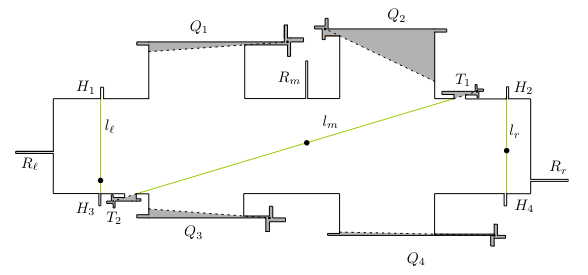
\includegraphics[width=0.7\textwidth]{Screenshot from 2022-01-21 12-46-51.png}
    \caption{Rectilinear Polygon $\mathcal P_R$}
    \label{fig:rectilinear}
\end{figure}
% a guard at position $x$ sees a point $y$ if the line segment $xy$ is fully contained in the polygon $\mathcal{P}$
% - a _guard set_ $S$ is a set of points in $\mathcal{P}$ s.t. every point in $\mathcal{P}$ is seen by some point in $S$ - find a minimum cardinality guard set for a simple polygon $\mathcal{P}$ on $n$ vertices
% - research less focussed on the classical problem, but more on its variations
% - no combinatorial algorithm for finding an optimal solution, or even for deciding whether a guard set of a given size $k$ exists, only real algebraic geometry powerful tools - not known if in NP
% - given polygons by integer coordinates, do they require guard positions with irrational coordinates in any optimal solution?
	% => yes, by constructing a _monotone_ polygon ($\exists$ line $l$ s.t. every line orthogonal to $l$ intersects $\mathcal P$ at most twice) with integer coordinates that can be guarded by three guards only when we allow to place the guards at points with irrational coordinates; otherwise, 4 guards are needed
			% - *place pic*
			% - **forcing a guard on a line segment** by creating 3 triangular pockets *pic* that can enforce 3 guards on 3 line segments within $\mathcal P$ - a guard can see both $t$ and $b$ if it is on the blue line segment $tb$, which is the intersection of 2 regions => $k$ pairs of triangular pockets and no 2 regions corresponding to different pairs of pockets intersecting => in order to guard the polygon with $k$ guards, there must be one guard on the line segment corresponding to each pair
			% - **restricting a guard to a region bounded by a curve** - consider a fixed position of $g_2$ on or to the right of the segment $bd$. $\exists$ a position of $g_1$ on $l$ s.t. the entire polygon is seen by $g_1$ and $g_2$ iff. $g_2$ lies on or to the left of the curve $\mathcal C$ *insert pic*
			% - **restricting a guard to a single (irrational) point** - *insert pic* $g_m$ and $g_l$ can guard together the 2 left pockets, and at the same time $g_m$ and $g_r$ can guard together the two right pockets => $g_m$ can only be in the irrational point $p = (3.5 + 5\sqrt 2, 1.5\sqrt 2)$
			% - **searching for the polygon** - we need to force $g_m$ to be on a line $l_m$ containing $p$, but we can only force $g_m$ to be on a rational line => we require the existence of a rational line $l_m$ that contains $p$ - there can be at most one rational line containing the irrational point $p$, as any 2 rational lines intersect in a rational point => reverse-engineer the polygon, after having chosen the positions of the guards of the form $(r_1 + r_2\sqrt 2, r_3 + r_4\sqrt 2), r_1, r_2, r_3, r_4 \in \mathbb Q$ ; rectangle with pockets added
	% - consider any set $S$ for $\mathcal P$ consisting of at most 3 guards: then $|S| = 3$ and $\exists$ 1 guard on each of the lines $l_l, l_m, l_r$
	% - consider any guard set $S$ for $\mathcal P$ consisting of 3 guards; then 1 of the guards has an $x$-coord in $[10.5, 10.6]$. For the remaining 2 guards, $g_l$ has a $y$-coord in $i_1 = [0.5, 0.6]$ and the $g_r$ in $i_2 = [1.7, 1.8]$
	% - **dependencies between guard positions**
		% - the guards $g_l$ and $g_m$ together see all of $e_t^l$ and $e_b^l$ and the guards $g_m$ and $g_r$ together can see all of $e_t^r$ and $e_b^r$ *add pic*
	% - **computing the unique solution**
		% - the max $x$-coord of $g_m$ s.t. $g_l$ and $g_m$ can together see $e_t^l$ and $e_b^l$ is $x = 3.5 + 5\sqrt 2$. The corresponding position of $g_l$ is $(2, 2 - \sqrt 2)$
		% - the min $x$-coord of $g_m$ s.t. $g_r$ and $g_m$ can see both $e_t^r$ and $e_b^r$ is $x = 3.5 + 5\sqrt 2$. The corresponding position of $g_r$ is $(19, 1 + \frac{\sqrt 2}{2})$  
	% - $\forall n$, there is a family of polygons $(\mathcal{P}_n)_{n \in \mathbb{Z}_+}$ which can be guarded by $3n$ guards with irrational coordinates, but need $4n$ guards to be rational; the coordinates of the points defining the polygons $\mathcal P_n$ are polynomial in $n$
	% - there is a rectilinear polygon $\mathcal P_R$ given by integer coordinates that require guards with irrational coordinates in any optimal solution - $\mathcal P_R$ can be guarded by 9 guards if we allow placing guards at points with irrational coordinates; an optimal guard set of $\mathcal P_R$ with guards at points with rational coordinates has size 10
		% - start with $\mathcal P$ - extend the non-rectilinear parts by "equivalent" rectilinear parts (gray) s.t. each of them requires at least  1 guard in the interior; if the interior of each pocket contains only 1 guard, then these guards must be placed at specific positions, making the area not seen by these 6 additional guards (white) => the remaining 3 guards must be placed at 3 irrational points (*place pic*)
% - _terrain guarding problem_ - $x$-monotone polygonal curve $c$ is given, the region $R$ above $c$ has to be guarded, and the guards are restricted to lie on $c$ - discretisation available in $O(n^3)$ time -> no irrational numbers phenomenon, and the decision version of the terrain guarding problem is in NP